\documentclass[conference]{IEEEtran}


\usepackage{amsthm}
\usepackage[cmex10]{amsmath}
\usepackage{amsfonts}
\usepackage{amssymb}

\ifCLASSINFOpdf
\usepackage[pdftex]{graphicx}
\usepackage{subfigure}
\else

\usepackage{graphicx}
\usepackage{subfigure}
\fi
\usepackage{epstopdf}
\usepackage{color}
%\usepackage[justification=centering]{caption}

\usepackage[font=normalsize]{caption}

\usepackage{algorithmic,algorithm}
\renewcommand{\algorithmicrequire}{\textbf{Input:}}
\renewcommand{\algorithmicensure}{\textbf{Output:}}
\newtheorem{theorem}{Theorem}
\newtheorem{lemma}{Lemma}
\newtheorem{remark}{Remark}
\newtheorem{proposition}{Proposition}
\newtheorem{corollary}{Corollary}
\renewcommand{\algorithmicrequire}{\textbf{Input:}}
\renewcommand{\algorithmicensure}{\textbf{Output:}}


\usepackage[numbers,sort&compress]{natbib}
\usepackage{color}
\renewcommand{\bibfont}{\footnotesize}

%\usepackage{hyperref}
%\usepackage{hypernat}

%\usepackage{cite}
%\usepackage{hyperref}
\usepackage{url}


\usepackage{mdwtab}

% correct bad hyphenation here
\hyphenation{op-tical net-works semi-conduc-tor equili-brium theo-retical calcula-ting func-tions}



\begin{document}
	
	\title{FlowCGAN: Exploratory Study of Class Imbalance for Encrypted Traffic Classification Using CGAN}
	
	
	% author names and affiliations
	% use a multiple column layout for up to three different
	% affiliations
	
	
\author{\IEEEauthorblockN{Pan Wang\IEEEauthorrefmark{1}, Shuhang Li\IEEEauthorrefmark{1}, Feng Ye\IEEEauthorrefmark{2}, 
		Zixuan Wang\IEEEauthorrefmark{1} and Moxuan Zhang\IEEEauthorrefmark{3}}
		\IEEEauthorblockA{
		\IEEEauthorrefmark{1}School of Modern Posts, Nanjing University of Posts \& Telecommunications, Nanjing, China\\
		\IEEEauthorrefmark{2}Department of Electrical \& Computer Engineering, University of Dayton, Dayton, OH, USA\\
		\IEEEauthorrefmark{3}Schools of International Education, Jinling Institute of Technology, Nanjing, China\\
		Email: \IEEEauthorrefmark{1}wangpan@njupt.edu.cn,
		\IEEEauthorrefmark{1}lish@runtrend.com.cn,
		\IEEEauthorrefmark{2}fye001@udayton.edu,
		\IEEEauthorrefmark{1}wangzx@runtrend.com.cn},
		\IEEEauthorrefmark{3}zhangmoxuan\_7@126.com}	
\maketitle
	
%Abstract	
\begin{abstract}
In the field of encrypted traffic identification, more and more researchers have begun to apply machine learning (ML), especially deep learning (DL) to traffic classification problems. Although these methods can automatically extract traffic features to overcome the difficulty of traditional classification methods like DPI in terms of feature engineering, a large amount of data is needed to learn the characteristics of various types of traffic. Therefore, the performance of classification model always significantly depends on the quality of the data set. The establishment of data sets is a time-consuming and laborious task. At the same time, it is often difficult to collect a large amount of traffic for some unpopular applications while traffic of hot applications is easy to access, which leads to the problem of data imbalances in data sets. In this paper, we proposed an unbalanced dataset solution based on FlowCGAN. As an instance of Generative Adversarial Nets(GAN), the method utilizes the advantage of GAN in data augmentation and generates new data samples by learning the characteristics of the traffic data, thereby achieving the purpose of balancing the data set. To verify the feasibility of this method, we use a classical deep learning model Convolutional Neural Networks(CNN) to classify the unbalanced data set, the random oversampled balanced data set, and the FlowCGAN balanced data set respectively. The experimental results show that the FlowCGAN method has better performance when compared with the other two data sets under the same conditions.
\end{abstract}

\begin{IEEEkeywords}
encrypted traffic identification, deep learning, Conditional Generative Adversarial Nets, traffic classification, data balance, convolutional neural network
\end{IEEEkeywords}


% Introduction
\section{Introduction}\label{sec:intro} % add a label for reference
As an important part of Smart Grid, IoT application mainly includes status monitoring of power transmission equipments and substation power environment, electric vehicle charging and discharging operational management, intelligent management of electric power supply, power asset management, electricity information collection, etc. In recent years, with the rapid development of Smart Grid and exponential growth of IoT nodes, e.g., smart meters, status monitoring sensors, traditional Cloud Data Center computing paradigm is unable to meet the requirements of IoT application in Smart Grid, including high bandwidth requirements, latency-sensitive and location-awareness. Fog Computing proposed by Cisco extends the Cloud Computing paradigm to run geodistributed applications throughout the network~\cite{bonomi2012}. In contrast to the Cloud, the Fog not only performs latency-sensitive applications at the edge of
network, but also performs latency-tolerant tasks efficiently at
powerful computing nodes at the intermediate of network. At
the upper layer of the Fog, Cloud Computing with data centers can be
still used for deep analytics.
% Related work (very briefly)
Many related works have been carried out recently. Mohammad Aazaml et al.~\cite{Aazam2014gateway} proposed a Fog Computing and Smart Gateway Based Communication for Cloud of Things.   Mohammad Abdullah Al Faruque et al.~\cite{Faruque2016energy} brought forward an energy management platform based on Fog Computing architecture. Mohamed Saleem Haja Nazmudeen et al.~\cite{Nazmudeen2016PLC} introduced a distributed processing framework for data aggregation based on fog computing architecture. Feyza Yildirim Okay et al.~\cite{Okay2016smartgrid} presented an Smart Grid model based on fog computing. The model is divided into Smart  Grid layer, fog layer and the cloud layer from bottom to top. Smart Grid layer mainly consists of smart meters, smart appliances and other intelligent equipments. The fog layer consists of multiple fog computing nodes. The cloud layer is mainly responsible for data storage, analysis and mining. Based on the concept of fog computing someone proposed a portable data storage and processing solution applying to Advanced Metering Infrastructure (AMI)~\cite{Yan2016AMI}. In addition, many research works about programming model about IoT application have been carried out in recent years. I.Satoh~\cite{Satoh2013} proposed a framework for data processing at the edges based on Mobile Agent and mapreduce. S.Cherrier et al.~\cite{Cherrier2011} introduced a distributed logic for IoT services based on OSGi to improve the modularizaion programming. K.Hong et al.~\cite{Hong2013} brought forward a programming model called Mobile Fog for large scale applications on IoT to try to develop IoT application by fog computing.
However, existing schemes proposed before can not meet the new requirements of IoT application in smart grid, especially distributed coordination between fog computing nodes.

%contribution of this paper
There are two main contributions in this paper. Firstly, we propose a new distributed Fog Computing architecture for IoT application in smart grid. To improve the application latency, we integrate distributed coordination capacity called FCC(Fog Computing Coordinator) in our architecture, which gather information of FC nodes in the same area periodically. In addition, FCC also devotes itself to assigning jobs to FC nodes so that all nodes can fulfill some complex tasks collaboratively. Secondly, a programming model is proposed to realize the architecture. 

%paper organization
The remaining of the paper is organized as follows. The new Fog Computing architecture is presented in Section 2. In Section 3, the programming model corresponding to the architecture is disscussed. Section 4 presents the evaluation of our architecture and programming model. Finally, Section 5 draws conclusion of this paper.

% new Fog Computing Architecture
\section{Fog Computing Based Architecture for IoT application in Smart Grid}
\subsection{The new requirements for IoT application in Smart Grid}
In this section we will identify several requirements that
need to be taken into consideration to effectively deploy IoT
application in Smart Grid.
\subsubsection{Latency Sensitivity} Many IoT applications in Smart Grid  depend on instant decisions and even second level latencies are not tolerable~\cite{Chen2017}. For example, electric substations in smart grid systems are equipped with various sensors to monitor status of power transmission. In this scenario, any latency may lead to serious accident like power failure.
\subsubsection{Distributed Coordination} There are always a lot of sensors distributed in geographic area, e.g., charging piles for electric vehicles. It is very important that coordinating multiple sensors or nodes distributed in several areas to provide electric vehicles charging services of IoT application in Smart Grid. 
\subsubsection{Locations awareness and Mobility Support} In many IoT applications end devices of Smart Grid are mobile and geographic distribution such as electric vehicles. As the main goal of the Fog Computing is to move computing power close to where the data is generated, it is necessary to be able to aggregate data at the closest network element while the end devices are moving.


\subsection{Fog Computing Based Architecture for IoT application in Smart Grid}
As shown in Fig.~\ref{fig:Fig_1_architecture}, our fog computing based architecture for IoT application in smart grid is still divided into terminal layer, fog layer and cloud layer from bottom to top. 
\subsubsection{Terminal nodes layer} This is the bottom layer which is made up of smart devices, which are responsible for sending raw sensed data and event logs to upper layer.
\subsubsection{Fog layer} The middle layer consists of fog nodes deployed at the edge of network to extend the processing ability of cloud center. Compared with the traditional Fog Computing model, our fog layer is divided into fog nodes( FN ) sub-layer and fog nodes coordination( FNC ) sub-layer. With the ability of computing and storage, these fog nodes of FN sub-layer provide a mechanism for migrating processing logic to the edge of the network. The FN sub-layer also has the aggregation capability for the sensed data from terminal nodes layer. After gathering and analyzing raw sensed data, part of them directly feed back to the active nodes in terminal nodes layer to complete the real-time response and process to the emergency event, the other part is transmitted to FNC sub-layer. FNC sub-layer consists of multiple coordinators located in the geographical areas. Fog nodes are divided into several clusters, where there are a few equipments  with computing and storage selected by some principle. We call this equipments FCN(Fog Computing Coordinators), which focus on coordinating the fog nodes to deal with some complex tasks due to the problem of distributed collaboration during the service, for example, query a suitable charging station for moving electric vehicles. In addition to undertaking data analysis and processing of the sub-region, the coordinator is responsible for coordinating all fog computing nodes in the region to further improve application performance by using the parallel computing capabilities.
\subsubsection{The cloud layer} This layer is the upper layer in this architecture. It is composed of servers, such as Data Centers which are responsible for analyzing massive historical data. 


\begin{figure}[h]
	\centering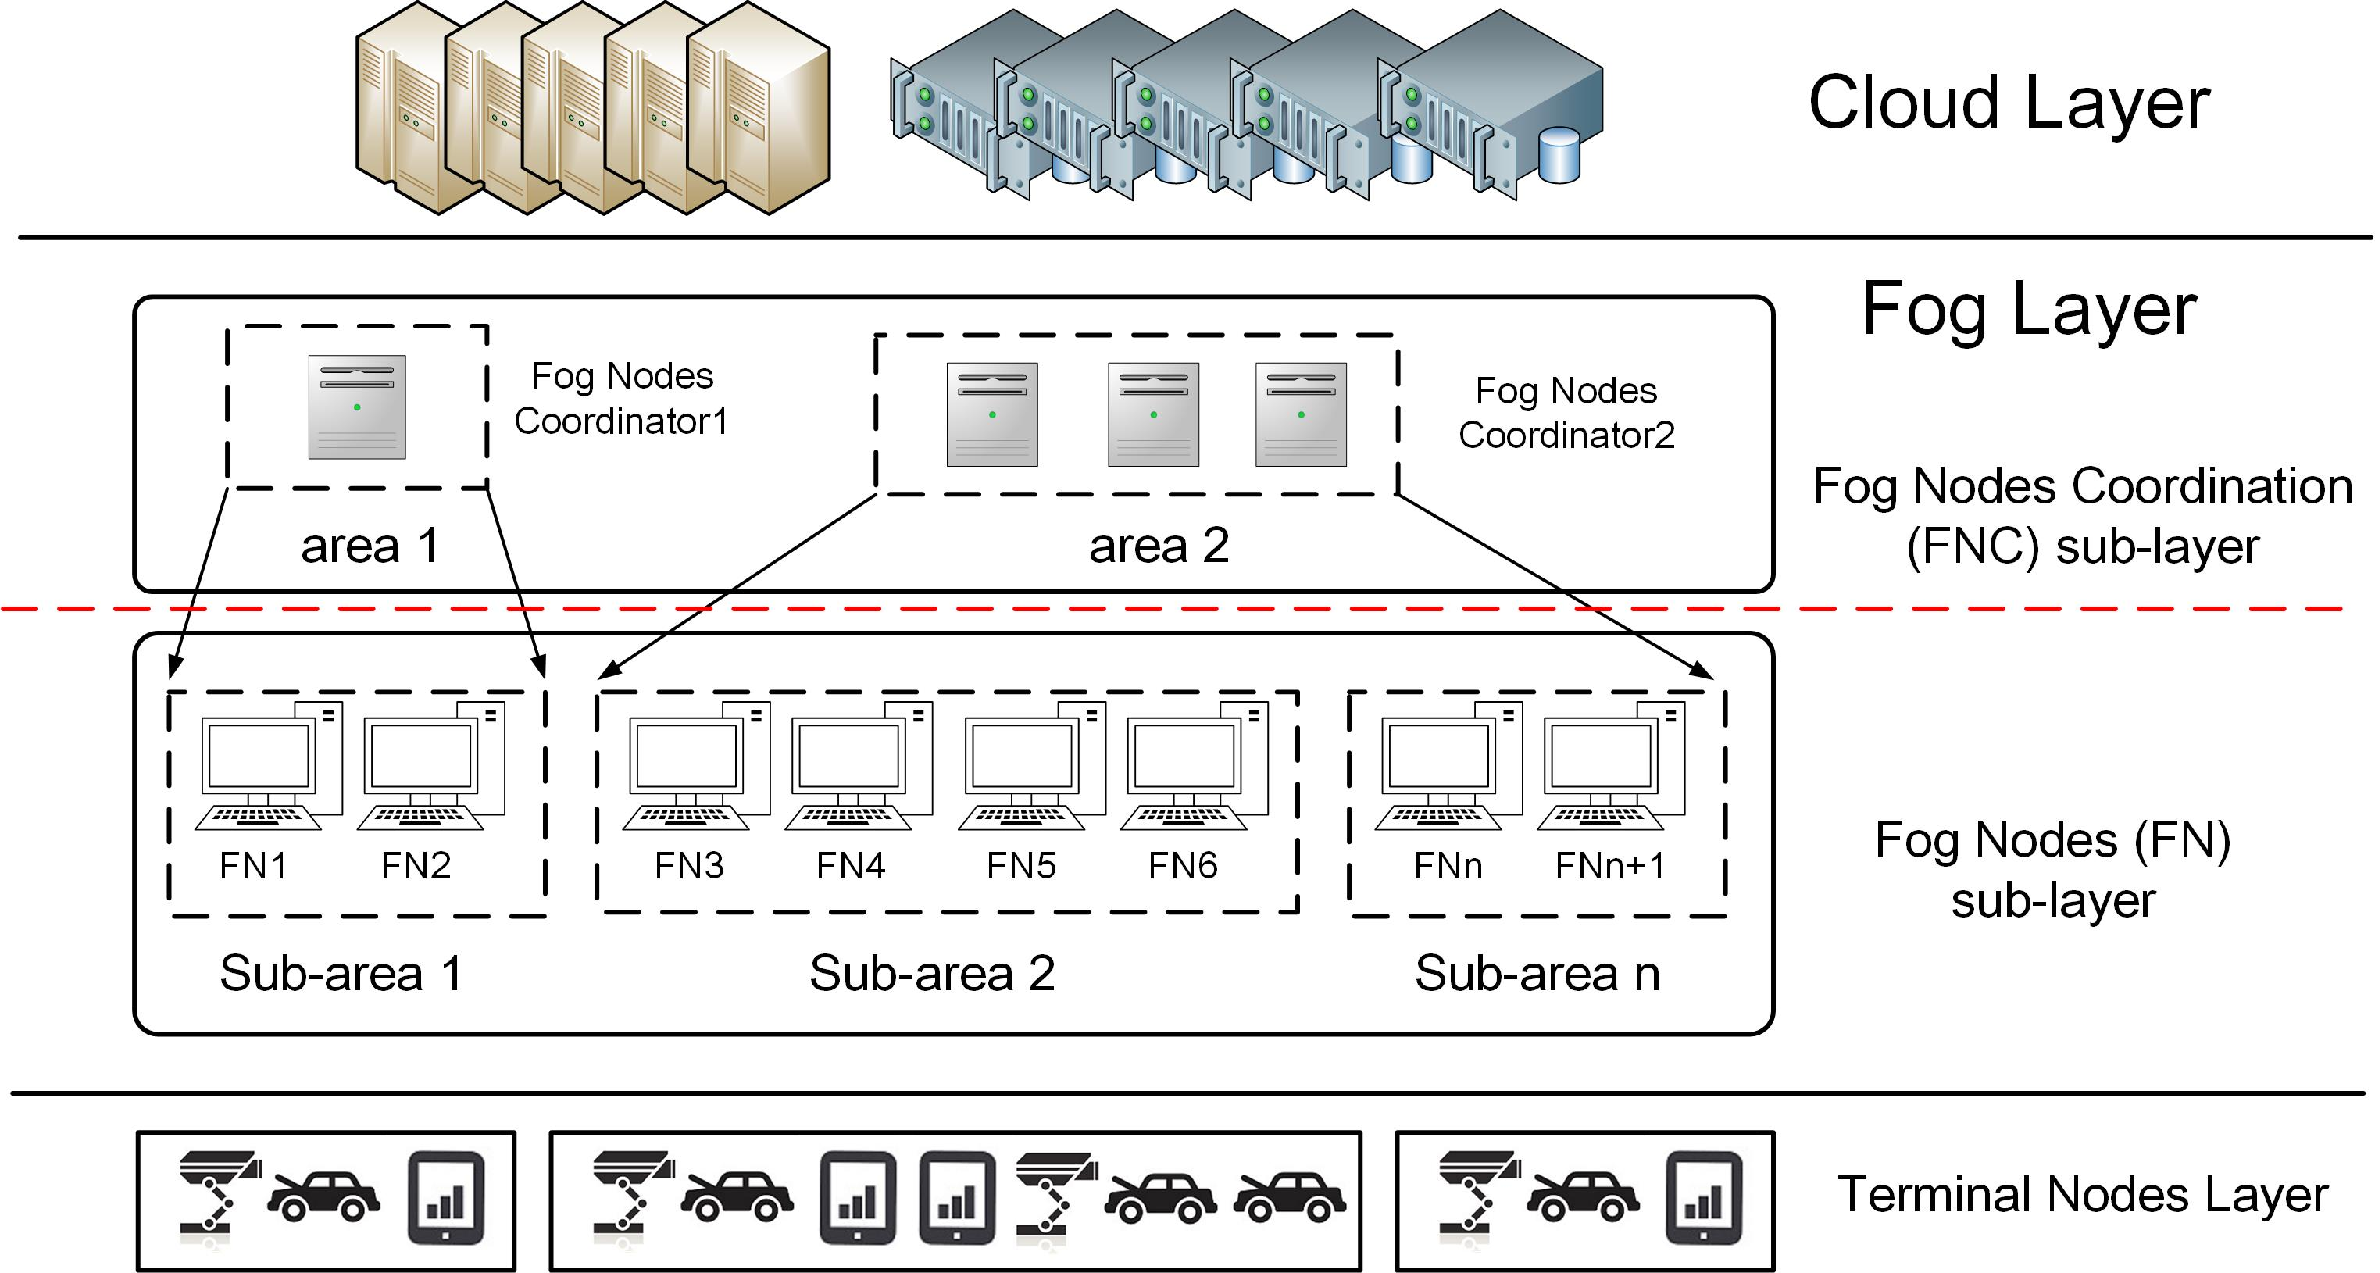
\includegraphics[width=3.4 in]{figures/Fig_1_architecture} 
	\caption{Fog Computing Based Architecture for IoT application in Smart Grid}\label{fig:Fig_1_architecture} % add a label for reference
\end{figure}




\subsection{System Model}
As shown in Fig.~\ref{fig:Fig_2_model}, the system model consists of sensors, action devices, communication nodes, fog computing nodes, cloud computing servers, FNC, service orchestration and scheduling servers called OSS servers. It is different with the system model proposed in papers, we introduce FNC sub-layer composed by FNC from each area. FNC accept requests from TN and decompose the services data flow according to the resource usage and service flow capacity of each FN and cloud computing servers, and then dispatch the jobs execution to related Fog nodes. Finally, FNC collect all the execution results to make the final decisions and instructions to the action devices. FN within the same layer have to achieve a complete user request under the coordination of FNC because there are no direct interaction between them. The interaction between FN and FNC can be realized by the way like relay communication, or Flow Table in SDN controller~\cite{Yiming2016}. 

Besides, we introduce OSS servers in Cloud Computing Center, which are able to decompose services data flow based on resource usage and capacity collecting from computing nodes. OSS servers dispatch job execution images to computing nodes by the way like traditional virtual machine with better security isolation or Docker container~\cite{Hong2016} with less start latency. OSS servers mainly aim at initialization deployment of new applications provided by service providers and setup service related execution logic on computing nodes. In contrast, FNC provide application services that meet the functionality and QoS requirements for end users by resource allocation and service logic coordination deployed in various computing nodes after receiving service requests from end users.   
\begin{figure}[h]
	\centering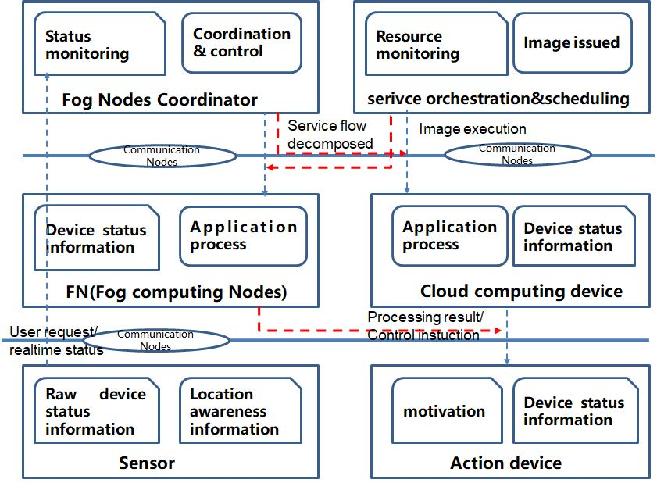
\includegraphics[width=3.4 in]{figures/Fig_2_model} 
	\caption{system model}\label{fig:Fig_2_model} % add a label for reference
\end{figure}



% Programming Model
\section{Programming Model}
\subsection{Programming Model Introduction}
The IoT application in Smart Grid can be considered as a distributed  application system essentially. However, the traditional programming model of distributed system was based on the model of "request-response" message interaction, which cannot meet the requirements of realtime processing  large amount of data generated by devices. Therefore, we need to design a programming model based on Data Flow programming~\cite{Johnston2004}. The typical programming framework is WoTKit processor based on WoTKit platform~\cite{Blackstock2012} and NR of IBM~\cite{ibm}. WoTKit is developed on JAVA Spring framework. Developer can run data flow program by creating wire between modules. However, WoTKit is designed for deployment of server level, it is better that using NR framework in IoT application, which was designed for application development in single computing unit, including nodes of input, output, processing and visual developing environment based on Web.In this paper~\cite{Giang2015}, author added some feature about distribution to  the traditional NR framework so that a data flow can be deployed in several computing nodes in the manner of multiple data flow slices. 
\subsection{Distributed Coordination Dataflow Programming model}
Distributed Coordination Dataflow Programming model is shown in Fig.~\ref{fig:Fig_3_programmingmodel}. Under the control of FNC, cloud servers and FN distributed in different geographic area together accomplish data analysis and processing of application services. There are two types of computing nodes, one is FN with rich computing resource,which choose Node-Red as distributed data flow computing framework. The other is FN with limited resource, which choose uFlow~\cite{Szydlo2017} as flow processing framework.

There are resident processes in every distributed computing nodes, which are responsible for collecting information like resource and capacity and then reporting to upper layer so that FNC will make better decision and instruction. After receiving substream and data ready to process, FN translate these data flow into instructions that can be identified and executed in terminal nodes. For example of parking service of electric vehicles, when a vehicle under the control of a sub-area FN apply a vehicle parking service, FNC of this sub-area will dispatch the request to all FN of this sub-area. After distributed coordinative processing of all FN, FNC can provide a best parking information for vehicles. As for online monitoring service all the time, we should consider the collaboration of Cloud Layer.After processing of FN in local area, FNC should report all the statistical data to cloud servers for future analysis.
\begin{figure}[h]
	\centering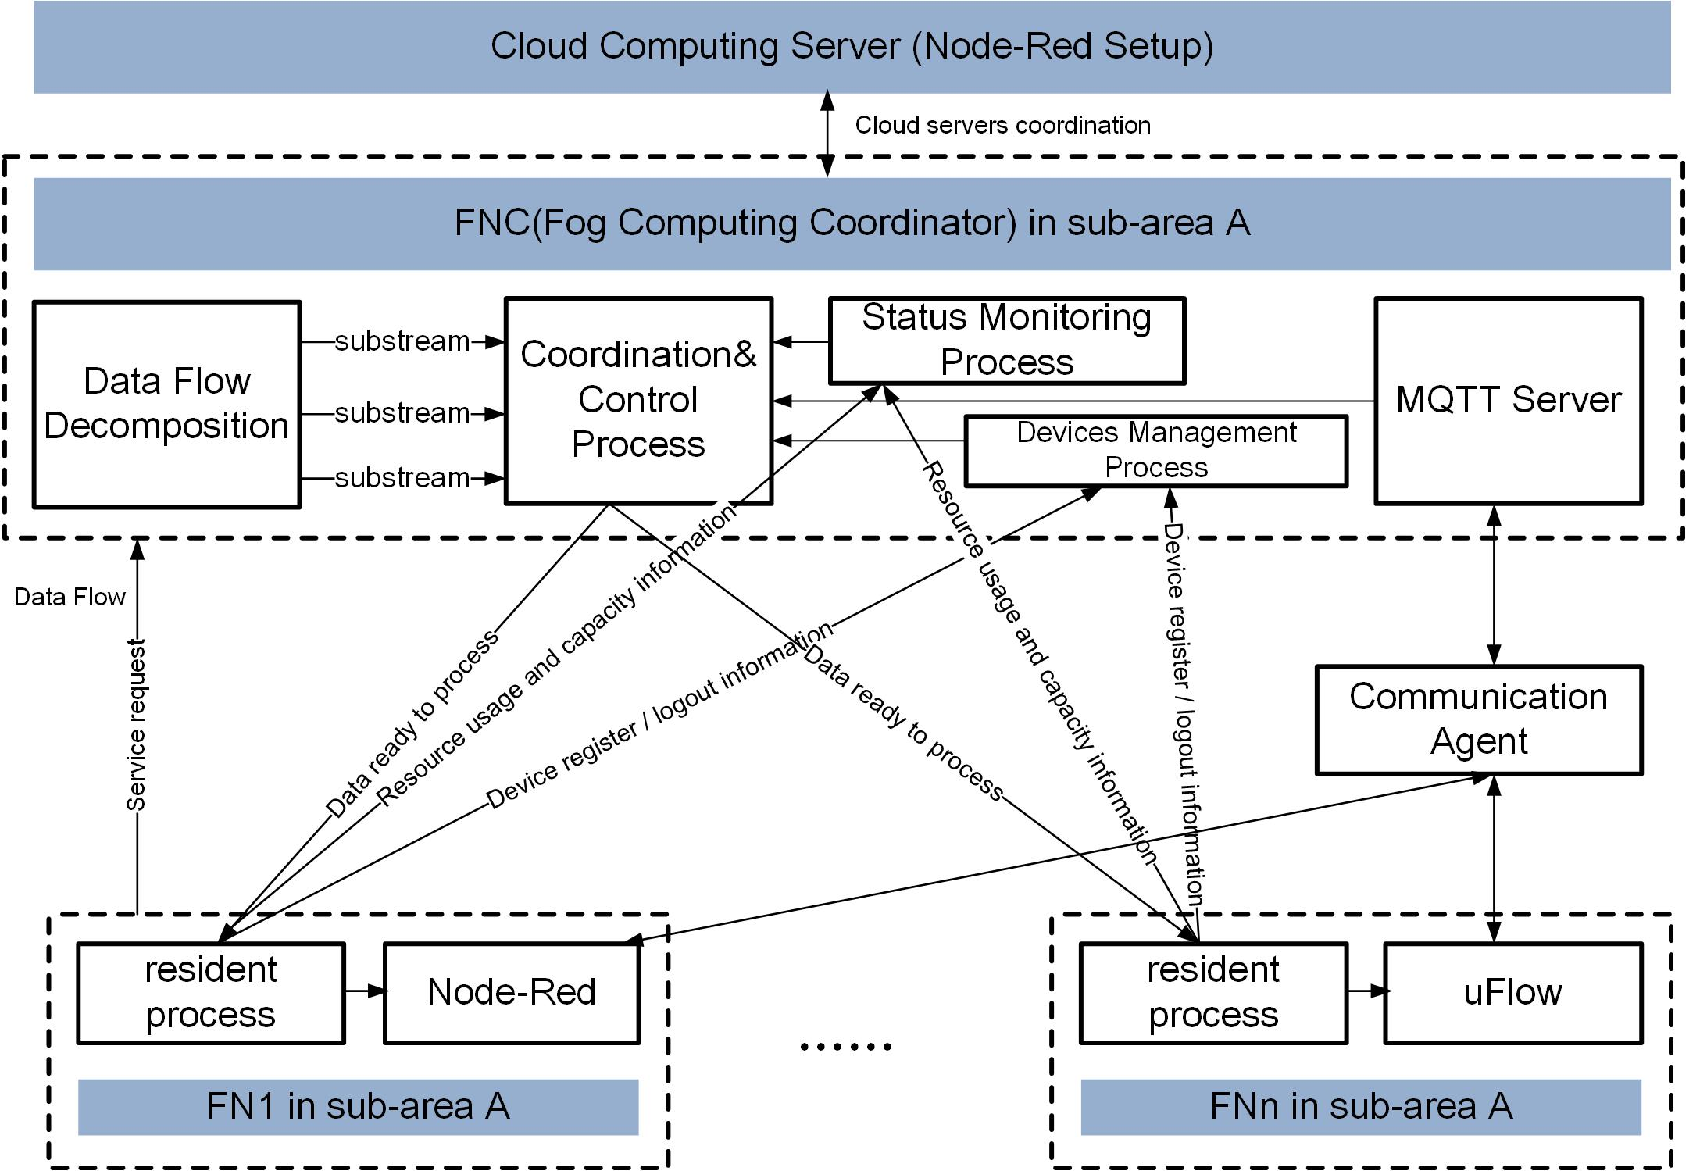
\includegraphics[width=3.4 in]{figures/Fig_3_programmingmodel} 
	\caption{programming model}\label{fig:Fig_3_programmingmodel} % add a label for reference
\end{figure}

Because of mobility of Terminal Nodes, the final data flow made by FNC may not suitable to current network condition, FN need coordinate themselves to adapt this situation at that time. That is called Fog Computing Nodes Migration. According to the initiator of migration, we can devide the migration into two types: one is initiated by FN; the other is Terminal Nodes. Two API used during the process of migration are following: 

1)State on\_migration\_start(nodeID): Invoked by migration device before migration process start. It returns a state object for flow information waiting for migration.

2)Void on\_migration\_end(state\_s): Invoked by migration target device after receiving request message from migration initiator.

The following is pseudocode describing the migration process for example of FN initiator.

1:  procedure migration\_source(nodeID)

2:   	obtain the actual latency T to node whose ID is nodeID

3:   	compare T with threshold Tupper

4:   	if  T  less than  Tupper

5:      	return;

6:   	else 

7:      	obtain the best candidate Vb from candidate group V

8:      	V = V - Vb

9:      	send a Start Migration message to node Vb

10:     	wait for response Resp

11:     if  Resp is ACCEPT then

12:        S = on\_migration\_start(nodeID)

13:        send Object State message to node Vb

14:        release local resource of dataflow relate to nodeID

15:        return

16:     else 

17:        if V is empty

18:          warn the message(can not migrate)

19:          return

20:        endif

21:     endif

22:     goto 7

23:  endif

24: end procedure

Compared with QoS of Terminal Nodes and FN's default threshold during process of substream computing, FN will decide whether migrate or not, see line 2-5.The detail are following: 1) choose the best nodes from node group with proper capacity, resource and QoS requirements, see line 7-8; 2) Send a migration start request message to alternative nodes and wait for response, see line 9-10; 3) if alternative nodes accept, then call on\_migration\_start to get all status information of current nodes and send to alternative nodes. Meanwhile, free all related resources of data flow ready to migrate, see line 11-15; 4) if alternative nodes do not accept, send the warning message,like can not migrate, and quit. Otherwise, choose the next alternative node from node group and repeat above-mentioned. target nodes will call on\_migration\_end to take over following work after receiving migration status message from migration initiator.

% Evaluation
\section{Evaluation}
\subsection{Simulation Setup}
The electric vehicle intelligent service system is composed of electric vehicle, charging pile, regional coordinator, regional application server, cloud service center, communication proxy server and basic communication network. As sensing devices of network at the edge of network, electric vehicles report relevant realtime information and request for services, as well as to provide services to users. The charging pile device is located at the edge of the network as a fog computing device. It processes the data according to the established application logic, and transfers the processed data through communication proxy server to application server of the region or romote cloud service center according to control of area coordinator. The regional application server joined with cloud service center provides related services to users. The difference is that the regional application server is more emphasis on providing some geographically related or strict requirements of delay services (such as navigation, intelligent parking, etc.), and the cloud center server provides some long-term analysis and forecasting services. According to density of charging pile and the size of traffic flow, we set a certain service area, and set up a regional coordinator in each area. The coordinator completes the data flow chart and transmits datas to relevant devices according to the service requests from users and the resources, capabilities, location information reported by the equipments.It coordinates these devices to complete the related service logic. For services that require cross-domain provisioning, coordination is done by regional application servers in different regions.

This section provides an electric vehicle intelligent service experiment system which is used to simulate and analyze the performance of the fog computing architecture presented in this paper. This paper chooses IBM's NR framework as an implementation tool for application development, and deployes a stream-based micro-runtime environment uFlow over resource-limited IoT devices. In the uFlow environment, we use Lua as the programming language, MQTT as a communication protocol. 
In this experiment, in order to supply charging service to the electric vehicle, the system selects the most suitable charging pile to the electric vehicle. There are two cases: one is based on the traditional fog computing architecture, in this case electric vehicles directly transmit the requests to all charging piles in a certain range, after the calculation, the charging pile met returns the confirmation to the electric vehicle. The other case is based on the fog computing coordinator architecture, in this case electric vehicles will directly send requests to the fog computing coordinator in the area. According to the information of the charging piles, the coordinator will forward the request to some charging piles with the possibility of providing the service and then the response is returned to the electric vehicle by the final eligible charging pile.

\subsection{Simulation Results}
The experimental system is mainly used to evaluate the contrast of application latency between the traditional fog computing architecture and our architecture based on fog computing coordinator. We used 20 software terminal nodes running on embeded system as electric vehicles, 10 software Fog nodes as charging piles and 2 FNC nodes. The range of all entity is located about 2000 meters. Fig.~\ref{fig:Fig_4_queryrange} shows the relationship between the application latency and the query distance of the two architectures. Clearly, it can be seen that when the query distance is short, the application latency is similar. However, when the query distance is gradually increased, our architecture has a lower application latency. In Fig.~\ref{fig:Fig_5_requests}, we discuss the relationship between the application delay and the number of service requests from the electric vehicles. Obviously, as the numbers of service request increase, the proposed architecture delay is significantly smaller than traditional one. Fig.~\ref{fig:Fig_6_FCN} describes the relationship between the number of fog computing coordinator and application latency. When the numbers of coordinators increase, the application latency decrease significantly. As shown above, the proposed architecture effectively reduces the application latency of IoT application in smart grid.
\begin{figure}[h]
	\centering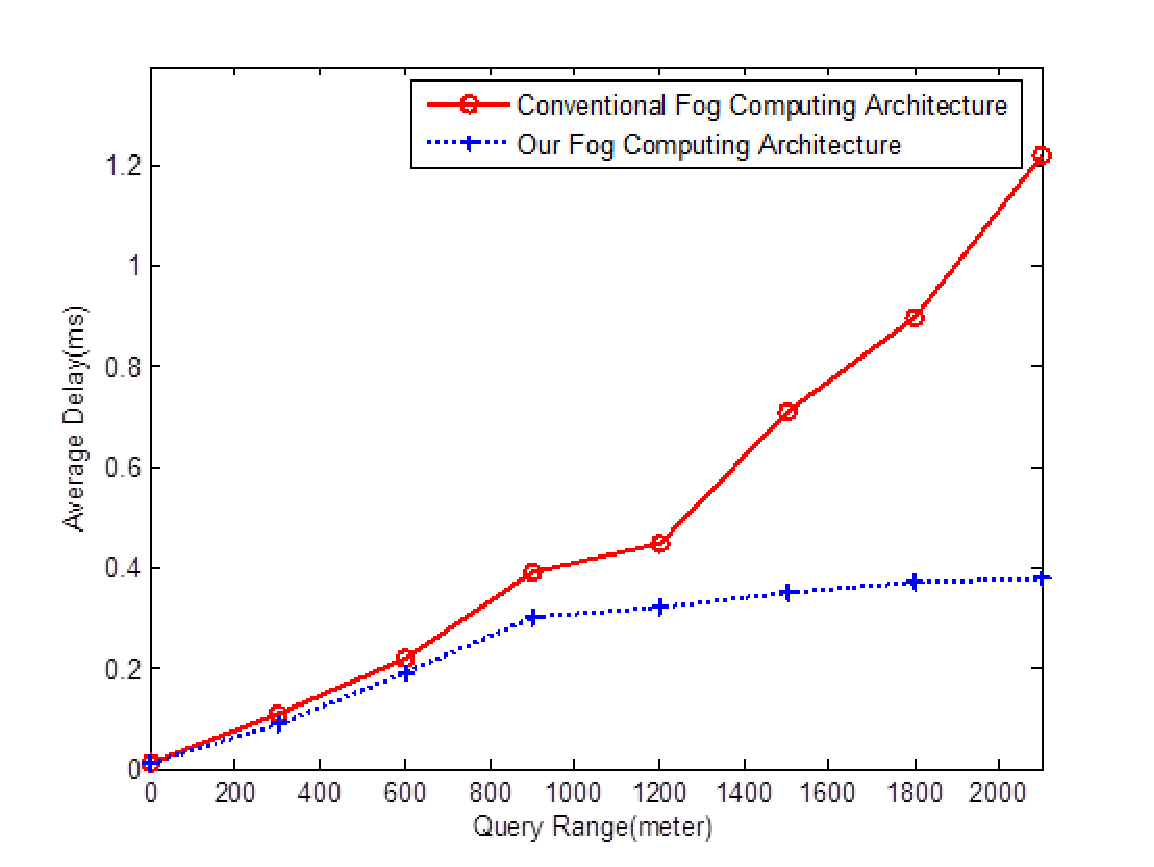
\includegraphics[width=3.4 in]{figures/Fig_4_queryrange} 
	\caption{application delay with query range}\label{fig:Fig_4_queryrange} % add a label for reference
\end{figure}
\begin{figure}[h]
	\centering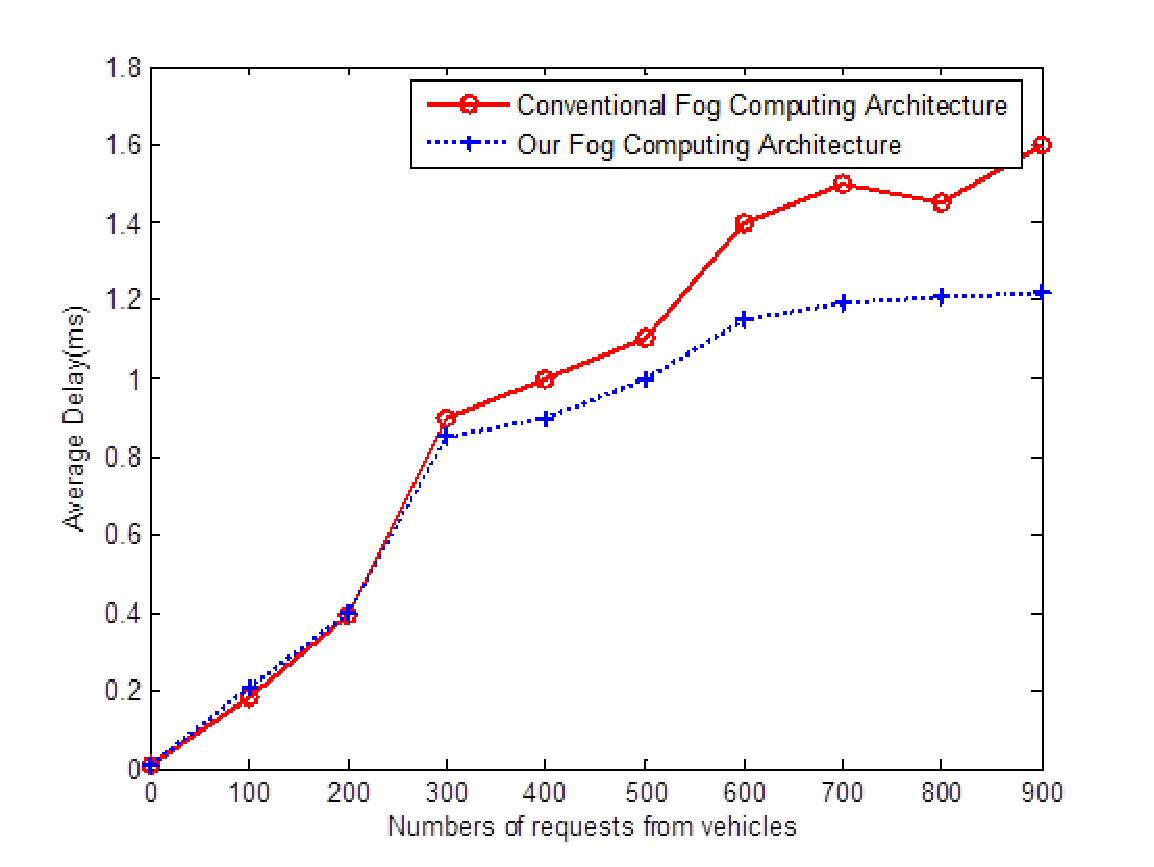
\includegraphics[width=3.4 in]{figures/Fig_5_requests} 
	\caption{application delay with service requests}\label{fig:Fig_5_requests} % add a label for reference
\end{figure}
\begin{figure}[h]
	\centering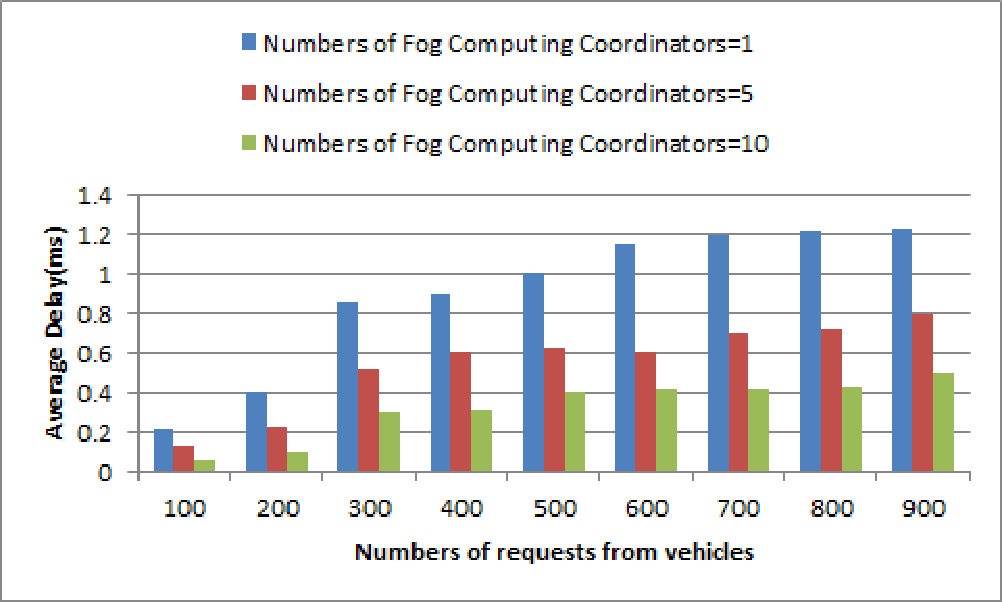
\includegraphics[width=3.4 in]{figures/Fig_6_FCN} 
	\caption{application delay with FNC}\label{fig:Fig_6_FCN} % add a label for reference
\end{figure}


% Evaluation
\section{Conclusion}
The IoT applications in Smart Grid need higher requirements in terms of response time and location-awareness. It can be met well by distributed computing architecture based on fog computing (edge computing) as a supplement to the traditional "cloud - link - end" architecture. In this paper, the proposed distributed fog computing architecture and programming model for IoT applications in smart grid can effectively reduce service latency. The application development in this paper is mainly based on the Data flow mechanism to realize communication between devices. Next we will find a more appropriate communication protocol; and study the optimization of resource allocation algorithm in this architecture. At the same time we will carry out the studies about the handover between the mobile nodes in high-speed mobility.





% Reference
% Please update the Reference.bib
\renewcommand\refname{Reference}
\bibliographystyle{IEEEtran}
\bibliography{IEEEfull,Reference}


\end{document}


